\section{Desarrollo}

\subsection{Ejercicio 1}
TODO: AGREGAR ALGO

\subsection{Ejercicio 2}
TODO: AGREGAR ALGO

\subsection{Ejercicio 3}
TODO: AGREGAR ALGO

\subsection{Ejercicio 4}
TODO: AGREGAR ALGO

\subsection{Ejercicio 5}

Los problemas que los autores estan intentando resolver en el paper el de programar varias tareas en un solo procesador en un contexto en el cual las tareas tiene asociado un deadline y hay que garantizar el cumplimiento de este último. \\

En el paper se limitan a analizar únicamente schedulers que utilizan prioridades y que adminten desalajo (preemptive) de tareas (En particular RM, EDF y una versión mixta).\\


El algoritmo de la sección 7 lo introducen por las limitaciones de RM.\\


La cota que definen los autores para poder saber si un conjunto de N tareas es factible para N grande es aproximadamente de $ln(X)$ es decir un poco menos del 70\% de utilización de CPU.
Es decir si el conjunto de N tareas utiliza aprox menos de $ln(X)$ de tiempo de CPU entonces se puede programar con RM cumpliendo los deadlines, si no cumple esa cota dependerá del conjunto y los periodos de las tareas para determinar si es factible o no. \\


El algoritmo de EDF proporciona una cota de factibilidad mucho mejor, si y solo si es factible programar un conjunto de tareas si su procesamiento no supera el 100\% de uso de CPU.\\


Esta cota de factibilidad de programación de tareas que tiene EDF implica que un conjunto de tareas puede ser programado respetando deadlines por un scheduler si y solo si EDF es capaz de hacerlo.\\


El teorema 7 deduce la cota de factibilidad de programación de un conjunto de tareas utilizando el algoritmo EDF.\\

Consiste en analizar el consumo de CPU que asigna a cada tarea el algoritmo EDF en un rango de tiempo grande. Sumando estos tiempos se obtiene el uso total de CPU asignado a tareas en ese rango. \\

La demostración de que si las tareas usan más del 100\% no se pueden programar con un solo CPU es simple dado que vale para cualquier scheduler, en ese sentido de la demostración ni siquiera usa que es EDF. \\

La demostración de que si las tareas tiene un consumo de CPU total no mayor al 100\% entonces se pueden programar con EDF es un poco más compleja y requiere de un teorema anterior de ese paper que dice que ''Cuando se usa EDF no hay tiempo desperdiciado (procesador IDLE) antes de un overflow (incumplimiento de deadline)''. Gracias a esta propiedad de EDF en el teorema 7 se demuestra (utilizando el absurdo) que se pueden programar las tareas.\\



\noindent
\emph{Diseño de SchedFixed:} \\

Se implemento con una cola de prioridad para los procesos listos, donde se asigno mayor prioridad a las tareas que tenían menor periodo (i.e. mayor frecuencia). 

Además generalizamos este algoritmo para más de un core y con desalajo por bloqueo.
Nota: Sabemos que no era necesario porque en el paper solo se menciona un core y un solo recurso el CPU.

Al programar mantuvimos el invariante de que en cada momento se trata de ejecutar la tarea de mayor prioridad comparando en cada tick la tarea que esta corriendo en el core con las que estan esperando en la cola de listos. En caso de encontrar una tarea más prioritaria en la cola de listo, se desaloja la que esta corriendo (Se hace un swap entre estas tareas).\\


\noindent
\emph{Diseño de SchedDynamic:} \\

Se implemento con una cola de prioridad para los procesos listos y adicionalmente con un map para guardar los deadlines, si bien el deadline se guarda en la cola de listos junto a su pid en una tupla, en cuando se necesita retirar de la cola de listos (ejemplo: cuando se bloquea o esta ejecutando en algún core) se guarda temporalmente en la otra estructura.

También en este caso generalizamos a varios cores e implementamos el desalojo por bloqueo.

Al programar mantuvimos el invariante de que en cada momento se trata de ejecutar la tarea cuyo deadline esta más próximo. Para esto se compara en cada tick la tarea que esta corriendo contra las tareas de la cola de listos, si se encuentra una que tiene deadline más proximo, se hace un swap de las tareas.\\


\subsection{Ejercicio 6}
TODO: AGREGAR ALGO

\subsection{Ejercicio 7}
TODO: AGREGAR ALGO

\subsection{Ejercicio 8}
TODO: AGREGAR ALGO

\subsection{Ejercicio 9}

Para mostrar con un ejemplo un caso que no sea factible para el scheduler RM y si lo sea para EDF nos basto el siguiente lote de 2 tareas periodicas:

Nota: Para simplicar el ejemplo consideramos en este caso despreciable el tiempo de cambio de contexto.
\\
\\
Lote:
\verbatiminput{graficos/lotes_ej9.tsk}

Produciendo los siguientes gráfico:

Para RM:

\begin{center}
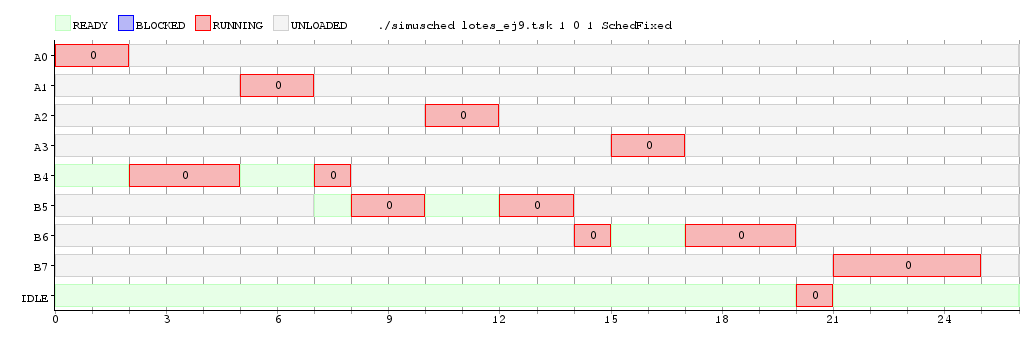
\includegraphics[scale=0.4]{graficos/eje9_fixed.png}
\end{center}

Para EDF:

\begin{center}
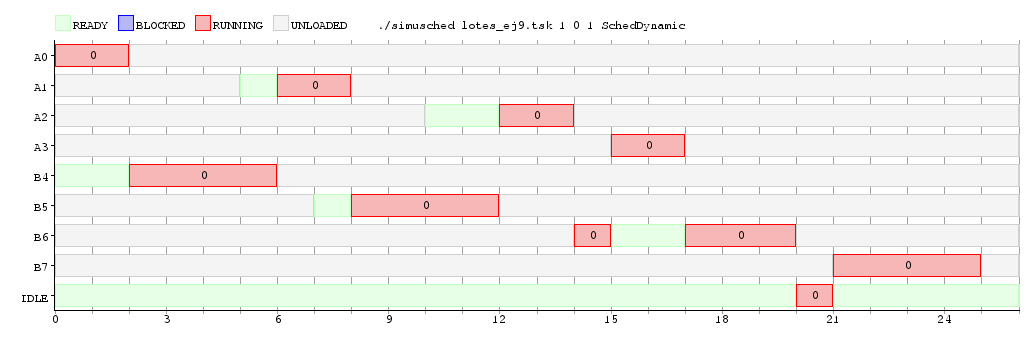
\includegraphics[scale=0.4]{graficos/eje9_dynamic.png}
\end{center}

La tarea de la familia A tiene un periodo menor que el de la familia B por lo cual según el scheduler RM tiene mayor prioridad asignada. Esta elección de priorizar a la familia A provoca un perjuicio en la familia B por lo que la familia B no puede cumplir su deadline en $T=7$ (Se produce un overflow).

En el caso del gráfico de EDF se puede observar que le da el CPU un poco más a la familia B por tener el deadline más próximo logrando evitar así el inclumplimiento del deadline (en $T=5$ deja esperando a la tarea de la familia A).

Algo interesante para destacar es que en este caso ambos scheduler ocuparon el mismo tiempo el CPU con trabajos, lo que cambia es que el scheduler RM a diferencia de EDF tiende a gastar más tiempo de computo en tareas de mayor prioridad dejandolo poco procesamiento a las de menor prioridad.

\subsection{Ejercicio 10}

En este caso encontramos un ejemplo en el cual las tareas son factibles tanto para RM como para EDF pero con un mejor uso de CPU por parte de EDF.

Nota: En este caso asignamos al cambio de contexto un costo 1.
\\
\\
Lote:
\verbatiminput{graficos/lotes_eje10.tsk}

Produciendo los siguientes gráficos:

Para RM:

\begin{center}
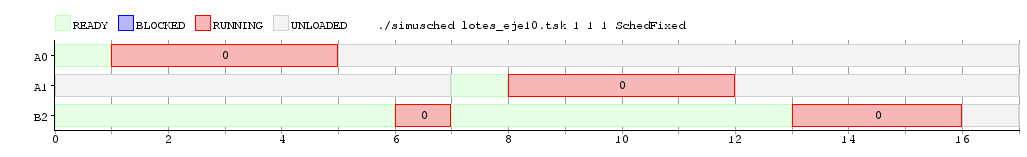
\includegraphics[scale=0.4]{graficos/eje10_Fixed.png}
\end{center}

Para EDF:

\begin{center}
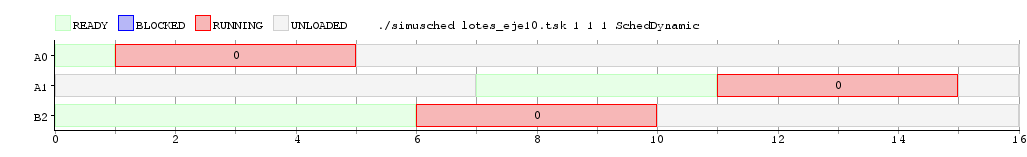
\includegraphics[scale=0.4]{graficos/eje10_Dynamic.png}
\end{center}

En este caso vemos que el scheduler RM necesita 1 cambio de contexto más que EDF lo que hace que el tiempo neto de procesamiento en tareas sea mayor en EDF (cambios de contexto con RM en T=\{0, 5, 7, 12\} mientras que EDF en T=\{0, 5, 10\}).

Intuitivamente se nos ocurre una conjetura para explicar este resultado, que sería que RM en general necesita más cambios de contexto porque toda tarea de menor prioridad es desalojada por las de mayor prioridad y como estas últimas tienen menor periodo (i.e. mayor frecuencia) la cantidad de desalojos es mayor.






